\chapter{Models for  Search-Encounter Data}
\markboth{Search-Encounter}{}
\label{chapt.search-encounter}

\vspace{0.3cm}


In this chapter we discuss models for search-encounter data. These
models are useful in situations where the locations of individuals are
observed directly by searching space in some fashion, rather than
biased by fixed trap locations. In most cases both detection
probability and parameters related to movement can be estimated using
such models. In the context of Bayesian analysis, we develop
search-encounter models conditional on movement outcomes, say
$u_{ik}$, the location of individual $i$ during sample occasion $k$.
The models we differentiate here depend on a number of things related
to data structure or survey protocol -- basically whether or not we
record the exact location and how we record it.

How exactly are search-encounter models different from models for data
from fixed arrays?  (1) sample units are either continuous space
polygons or lines, not points; (2) we have location information that
is not biased by trap locations (that is, restricted only to fixed
trap locations); (3) because we have direct observations of location
that exist independent of traps, we can often build an explicit model
of space usage or an explicit movement model.
% XXX RS: Couldn't you add your observation here, that with fixed arrays the movement model and the detection model are confounded? Actually, I think it might be necessary because we talk so much about movement models in the array models that without a little further info here it's not entirely clear why the movement models from search-encounter are different
Conversely, 
 when we have an array of fixed trap locations, the
movement process is completely confounded with the encounter process
because the list of potential observation locations is prescribed, a
priori, indendent of any underlying movement process.

A few distinct types of situations exist where these models come in
handy. The prototypical, maybe ideal, situation
\citet{royle_etal:2011mee} is where we have a single search path
through a region of space from which observations are made (just as in
the typical distance sampling situation, using a transect). As we walk
along the search path, we note the location of each individual that is
detected, {\it and their identity} (this is different from distance
sampling in that sense). 
Alternatively, we could delineate a search
area, and conduct a systematic search of that region. An example is
that of \citet{royle_young:2008}, which involved a plot search for
lizards. They assumed the plot was uniformly searched which justified
an assumption of constant encounter probability, $p$, for all individuals within the plot boundaries. 
The data set
was $\ge 1$ location observations for each of a sample of $n$
individuals.  The recent paper by \citet{efford:2011} discussed
likelihood analysis of similar models. In the terminology of \mbox{\tt
  secr} such models are referred to as models for {\it polygon
  detectors}.  The model described by \citep{royle_etal:2011mee} is a
generalization of the polygon search model, as we describe below.
% XX RS: You also gonna describe the transect model? Might be nice to add, if so. Something like in the other chapters, like, 'in this chapter... blabla'


\begin{comment}
%%## This argument here is basically true, but i'm not sure how to
%%package the idea yet.

Search-encounter models also provide something of a bridge between the
standard models for fixed trap arrays (e.g., Chapt. \ref{chapt.scr0}, etc.),
and the models described in Chapt. \ref{chapt.noID} in which individual
identity is not available. One one hand, in the standard fixed trap
array situation, we observe individual encounter data at each fixed
trap. In the ``no ID'' models, we observe trap-specific encounter
frequencies, but no individual identity. 
Search-encounter models are intermediate
in terms of the structure of the observable data.

\end{comment}


\section{Search-encounter sampling designs}

Before we discuss models for search-encounter data, we'll
introduce the types of sampling situations that
produce individual location data.  We imagine there are a lot more sampling protocols
than identified here, but these are some of the standard situations that we have
encountered over the last few years in developing applications of SCR
models.  For our purposes here we recognize 4 basic sampling designs,
each of which might have variations due to modification of the basic
sampling protocol. In later sections of this chapter we will explore some
examples involving of some of these situations. 

\subsection{Design 1: Fixed Search Path}
\label{searchencounter.sec.fixedpath}

The ideal situation is where we have a continuous search-path or
line, or multiple such lines, in some region
(Fig. \ref{searchencounter.fig.snakeline}). This is the type of
problem described by \citet{royle_etal:2011mee}. We assume the paths or
lines are laid out a priori in some manner that is done independent of
the activity centers of individuals and the collection of data does
not affect the lines.  That is, we assume the lines are established
{\it a priori} without consideration of factors that might affect
density. A situation in which this may be violated is when sampling is
based on sniffer dogs. A handler working a team of dogs is usually
letting the dogs ``follow their nose'', and the dogs are adapting to
their own senses as they work the landscape. 
In some cases the lines are within well-defined
polygons (shown in Fig. \ref{searchencounter.fig.snakeline}) but the
polygon boundaries may or may not be meaningful in terms of the
observation process. That is, if one is sampling along the path shown
in Fig. \ref{searchencounter.fig.snakeline} and recording locations of
individuals, then the boundary is not relevant if individual locations
may be recorded outside the polygon boundary. In this case, perhaps
the polygon boundary (quadrats in
Fig. \ref{searchencounter.fig.snakeline}) was used as a mechanism for
producing the transect, but does not affect the collection of data.  A
number of variations of this search encounter situation are possible,
and these produce slightly different data structures and corresponding
modifications to the model:
% XX RS: The list is not very intuitive. Why7when would we record the location on the transect where we first saw an individual? (1b) And in the CR-DS hybrid, don't wen use the distance to get at the location of the individual? I guess what's not quite clear here is: are these protocolls that lead to different data structures and thus, different models, or are these just different survey techniques to get at the same thing, namely individual locations
% Andy sez: Good point.  I added a phrase to above sentence but not
% sure what else to say. 
\begin{itemize}
 \item[] Protocol (1a). We know the search path and record the locations of individuals.
 \item[] Protocol (1b). We record the location of individuals and
   the location on the transect where we first observed the individual.
 \item[] Protocol (1c). We record
the closest perpendicular distance. This is a typical
   distance sampling situation, and this is a type of hybrid CR-DS model.
 \item[] Protocol (1d). In this case, observations are restricted to
   the line itself. We imagine that the line is evolving in response
   to search activity. 
 \end{itemize}


\begin{figure}
\centering
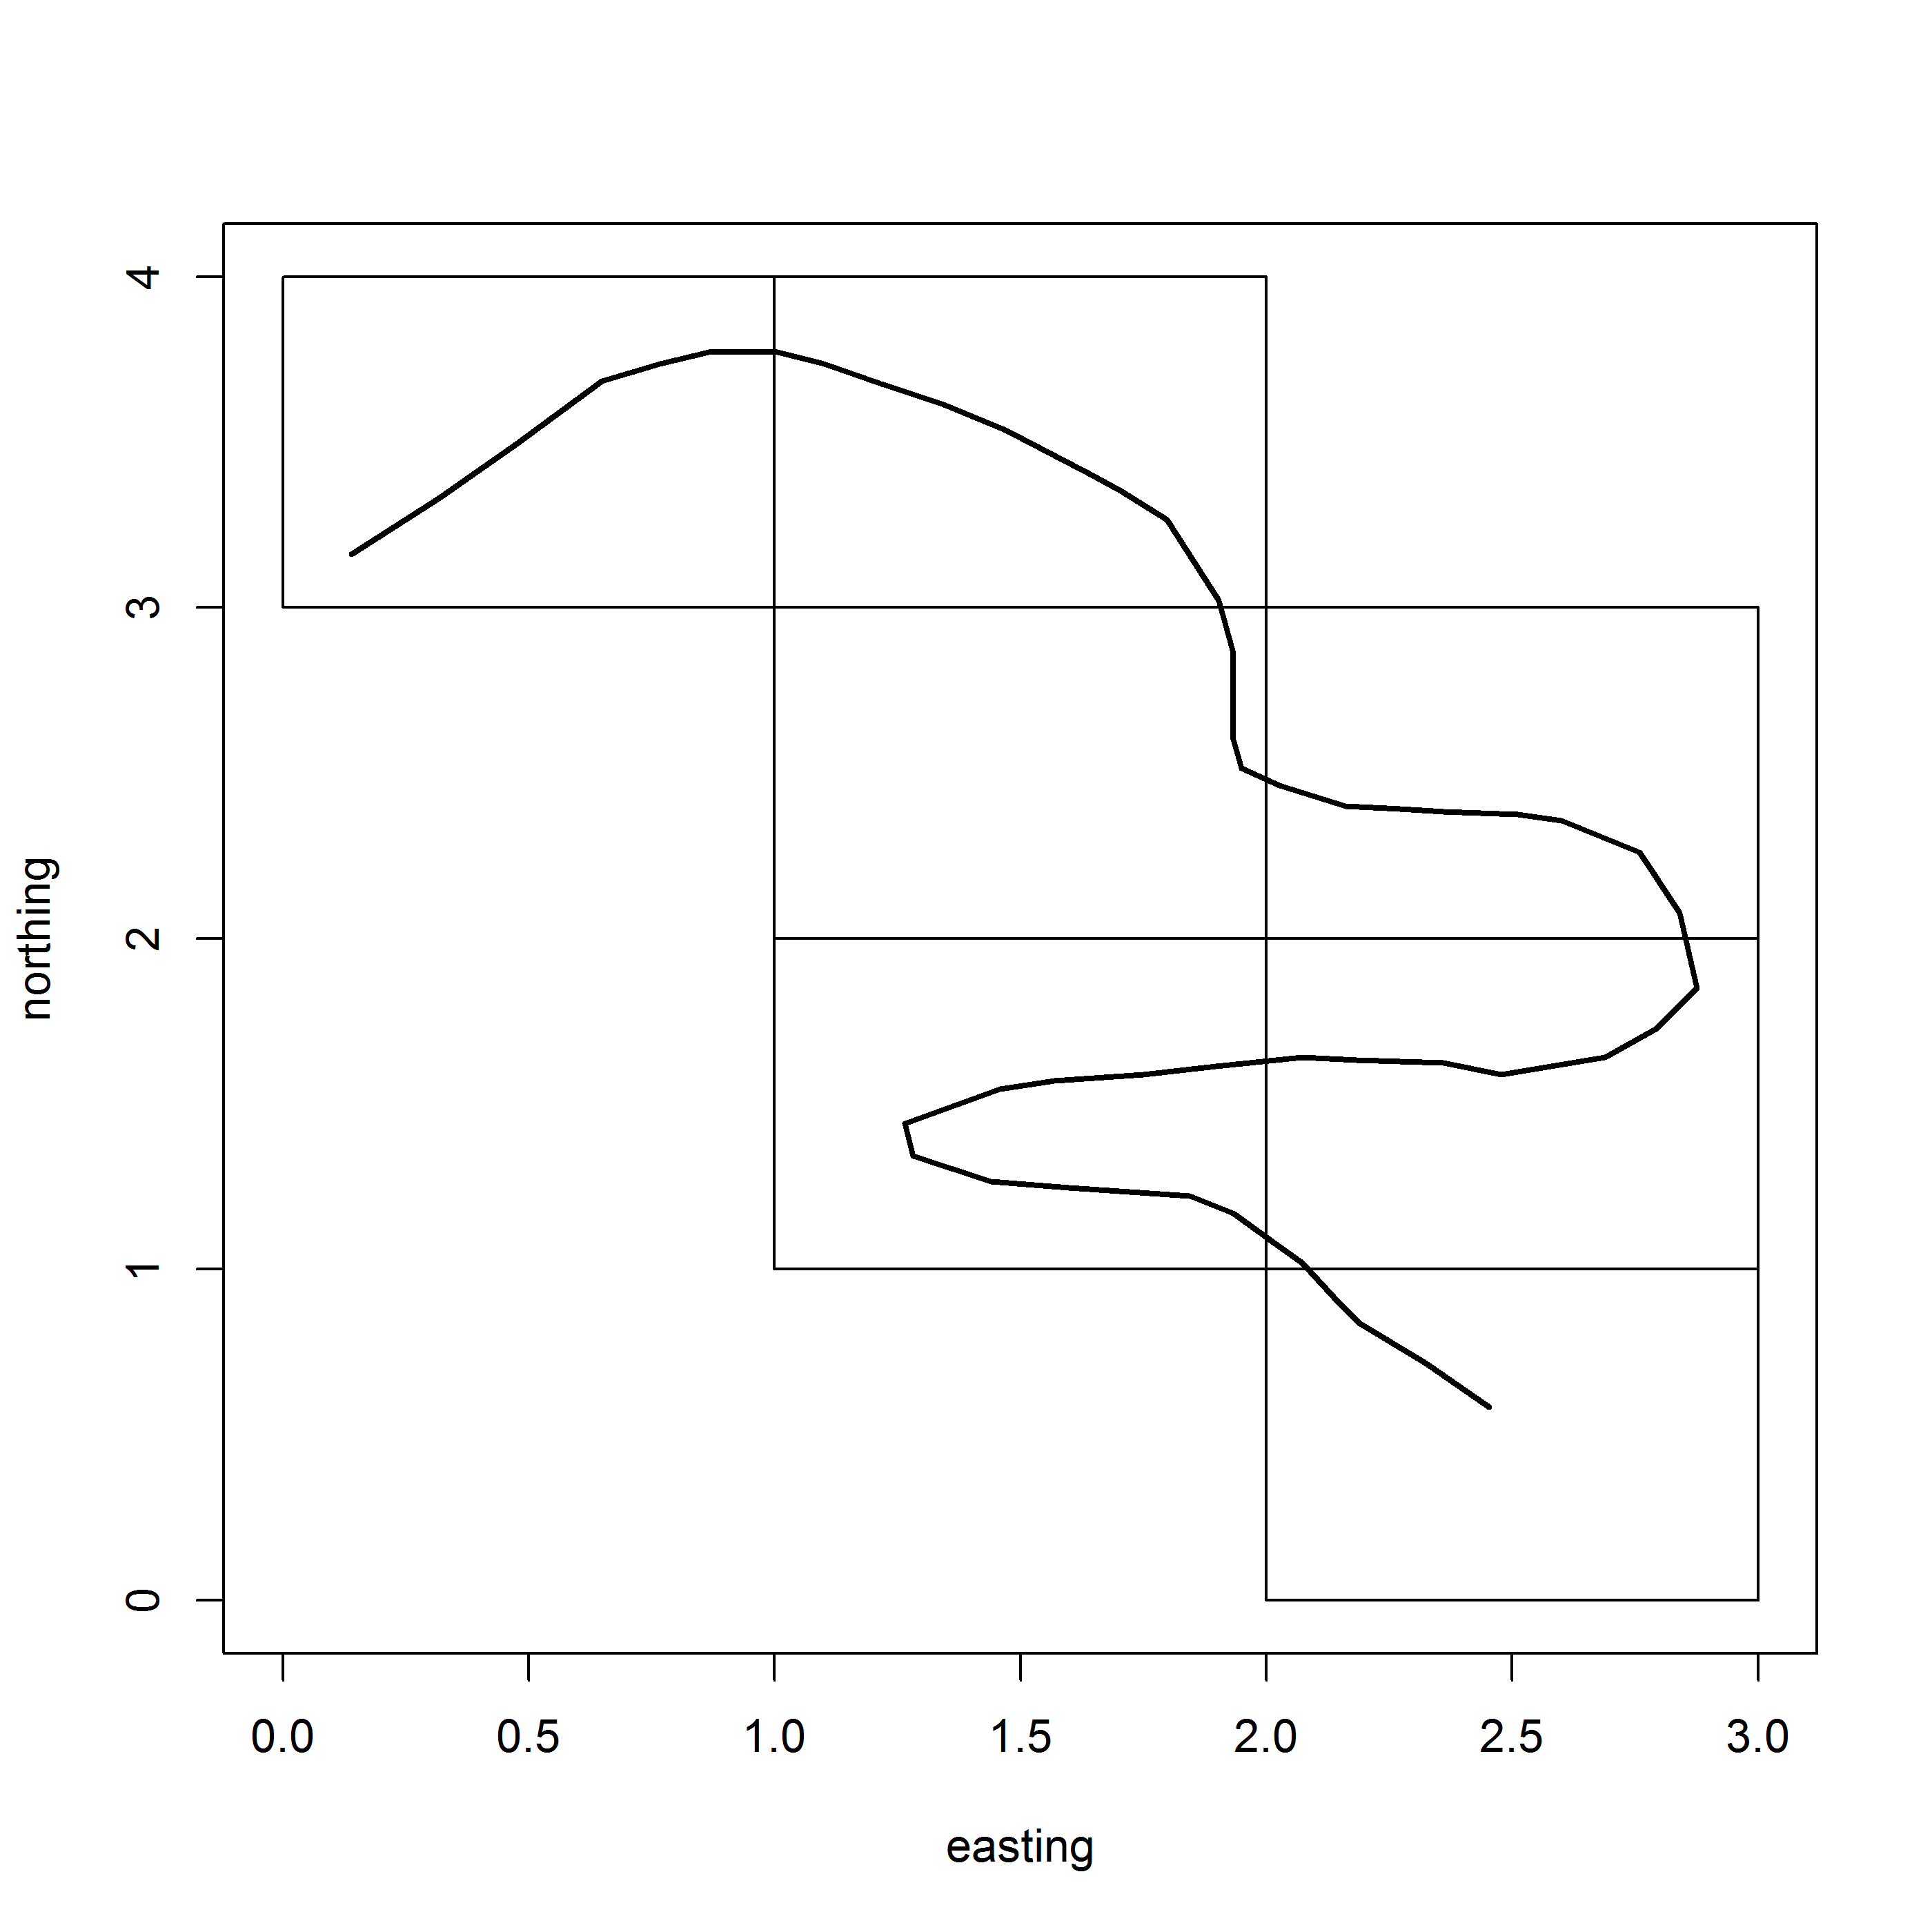
\includegraphics[width=4in,height=4in]{Ch15-searchencounter/figs/snakeline.png}
\caption{
A survey line through parts of 7 quadrats in a
  hypothetical landscape. An observer travels the transect and
  identifies individuals in the vicinity of the line, recording their
  identity and location.
}
\label{searchencounter.fig.snakeline}
\end{figure}


\subsection{Design 2: Uniform search intensity}

In this case we have one or more well-defined sample areas (polygons),
such as a quadrat or a transect, and we imagine that the area is
uniformly searched 
so that encounter probability is constant for all
individuals within the search area
(we'll abbreviate this as ``the USI model'').
 Sampling produces locations of
individuals within the well-defined boundaries of the sample area. The
polygon boundaries defining the sample unit are important because it
tells us that $p=0$ by design outside of the boundary.

Using the example from the Fig. \ref{searchencounter.fig.snakeline},
we imagine that each of the identified quadrats is uniformly searched,
which is to say, we assume that 
 each individual within the boundaries of the {\it quadrat}
has an equal probability of being detected.  In the context of
replicate sampling occasions (e.g., on consecutive days), individuals
may move on or off of the plot, and so individuals may have different
probabilities of being {\it available} to encounter, based on the
closeness of their activity center to the quadrat boundaries. However, given
that they're available, the USI model assumes they have constant
encounter probability. 
% XX RS: A couple of things here: I would point out that (if I
% understand that correctly) individuals don't have the same
% probability of being within the search path, though, because them
% being  there depends on how far away they live. Otherwise this
% statement is just a little confusing. 
% 
%% The other thing is: it is not really clear if you are referring to
%% the quadrats in the figure and are saying that these were searcher
%% uniformly (not along the line that snakes through the quadrats in
%% the figure, but actually uniformly), or that if you look at how
%% much of the line is in each quadrat, the amount of 'effort' is the
%% same - so search effort is distributed uniformly among the
%% quadrats. I think the confusion might come from talking about area
%% searches (so I am thinking about 2-d space) but then referencing
%% the search path (where I think 1-d). Maybe this section just needs
%% some definitions up front to make things clearer.
%
% Andy sez: I resolved these things I hope

In this USI situation, where we have contiguous quadrats,  the
individual quadrat boundaries are irrelevant as far as the model
specification goes,  and we
only need to be concerned about the ``total'' boundary of the
composite polygon (the intersection of all little ones). That said,
for analysis in {\bf BUGS}, it is easier to work with rectangular
polygons and so, from a practical standpoint, we might describe the
model in terms of each of the collection of smaller quadrats. It might also be advantageous
to ensure nice rectangular plot boundaries (or else write your own
MCMC algorithm, see Chapt. \ref{chapt.mcmc}).  We show a simulation
example for an area-search model below, and we analyze it both using a
bivariate normal model and a 2-d random walk type of model to describe
animal movement, i.e., the way individual locations ${\bf u}_{ik}$ are
generated. For further exampels and analyses, we refer you to
\citet{royle_dorazio:2008}, who reanalyzed the lizard data from
\citet{royle_young:2008}, and \citet{efford:2011ecol} and
\citet{marques_etal:2011}.

% XX RS: Would increase axis labels in the figure.
%% andy sez : needs done

\subsection{Partial Information Designs (3 and 4)}

In practice, we think many situations will arise in which partial
spatial information is available. The data structure and model are
slightly different in these cases.

{\bf Design 3}: We imagine that search polygons are defined
(e.g., the grid cells in Fig. \ref{searchencounter.fig.snakeline}) and
we record
locations of encountered individuals, but we do not perform a uniform search
of quadrats and we neglect to record the the search path. 
In this case, we don't have direct information on the observation
process -- we are not able to characterize the {\it probability of
  that specific observation} because, in general, it depends on the
precise configuration of the search path.  In this case, while it is
beneficial to have the location of the individual, we do lose some
information by not recording the points in space from which that
individual was detectable. This would be akin to neglecting to record
the trap locations in the standard situation of having a fixed array
of traps. 
% XX RS: It's not entirely clear to me: so we record individual locations, but we don't spread search effort uniformly and have no means of quantifying effort, is that it?I think it would help to be more explicit about why we need the search path, if we have the location of the individual, which is waht we're really interested in.
%% Andy sez: I embellished above. 

% XX RS - later: I understand now, but I think before or while you outline these protocols, it would be important to state what the different pieces are used for (without equations). So if we don't search an entire area, the path is essential because it tells us where we sampled and thus, where we were able to encounter individuals; also, the path locations are needed for the observation-by-distance model, if we want to specify one; and even if we assign detections to, e.g. grid cell centers, the path in each grid cell can tell us somethign about the search effort (analogous to how many days a camera trap was operational); and the locations of individuals are necessary to get at the movement model. Without these definitions it's hard to appreciate the differences in the data structure and they don't become fully clear until the end of section 2
What we have in these situations are
observations of individuals {\it and} the quadrat they were detected in,
but not the finer
scale ``movement'' outcomes.


{\bf Design 4}: In this we neglect to record a search line and also the locations of individuals
within the quadrats.  There are two variations of this:
\begin{itemize}
\item[] Protocol (4a) - You could have
counts by identified by individual within each quadrat. 
For example, if scats are collected and genetically assigned to individuals, and for each individual we get a count of scats in each quadrat.
\item[] Protocol (4b) - We don't have 
individual identities, but just total counts. This is the
\citet{chandler_royle:2013} model (Chapt. \ref{chapt.noID}).
\end{itemize}
It is possible also that we retain the survey line information, which
could possibly be used to identify a covariate of ``coverage'', in
order to account for different search effort in each quadrat.




\begin{comment}
\subsection{Examples}

The capricailie example: search of polygons -- could be search
encounter with uniform search intensity but we ignored the polygon
boundaries and just mapped each observation to the center point.  The
fisher data: we had a GPS line but it was not really fixed , it
evolved as dogs searched around. Therefore as a practical matter the
locations of samples were all {\it on} the line. We therefore mapped
to a center point of a grid. We make a grid of the sampled area and we
assume within each grid if a species is present then it is independent
.... actually if the grid is placed INDEPENDENT of the lines then its
probably safe to make some kind of independence assumption.  Russell
et al. -- similar situation, they have a search parth but not really
independent.

For the rest of this chapter, we will provide some model
formulations for some cases, provide code for simulating and analyzing
the data, and some real examples but not for every situation.
A number of published examples have been given. The Royle et al. 2011
paper on the MHB. The Royle and Young 2008 (see also Marques et
al. and Efford 2011). We also have the Thompson et al. XXX and Russell
et al. XXXX and Capricaillie paper XXXXX.

Possible examples to provide:

Example 1:  Analysis of the Swiss MHB survey using Design 1

Example 1b: Lizard data. No need to analyze this as it was done in RD book. Mention polygon detectors in secr.

Example 2: Fisher data possibly - lion data or -- or  Capricaillie data?
\end{comment}




\section{A Model for Search-Encounter Data}

We focus here on developing a model for Designs 1 and 2, as these
represent ideal sampling situations.  In contrast to most of the models
described in this book (but see Sec. \ref{poisson-mn.sec.acoustic}), we
develop models for encounter probability that depend explicitly on the
instantaneous location ${\bf u}_{ik}$, for individual $i$ at sample
occasion $k$: $p_{ik} \equiv p({\bf u}_{ik}) = \Pr(y_{ik}=1|{\bf
  u}_{ik})$.  Note that ${\bf u}$ is unobserved for the $y=0$
observations and thus we cannot analyze the conditional-on-${\bf u}$
likelihood directly. Instead, we regard ${\bf u}$ as random effects
and assume a model for them, which allows us to handle the
problem of missing ${\bf u}_{ik}$ values (Sec. \ref{searchencounter.sec.movement}).


To develop encounter probability models for this problem we cannot
just use the previous models because the ``trap'' is actaully a line
or collection of line segments (e.g.,
Fig. \ref{searchencounter.fig.snakeline}).  Intuitively,
$\Pr(y_{ik}=1|{\bf u}_{ik})$ should increase as ${\bf u}_{ik}$ comes
``close'' to the line segments ${\bf X}$. It seems reasonable to
express closeness by some distance metric $||{\bf u}_{ik} - {\bf X}
|| = dist( {\bf u}_{ik}, {\bf X})$ and then assume
\[
\mbox{logit}(p_{ik}) = \alpha_{0} + \alpha_{1} ||{\bf u}_{ik} - {\bf X}||.
\]
For the case where ${\bf X}$ describes a wandering line, some
kind of average distance from ${\bf u}$ to the line
might be reasonable; possible alternatives include the absolute
minimum distance or the mean over specific segments
of the line (within some distance), etc.  We could also have a model
without an explicit distance component, by assuming that individuals
within a certain distance from the search path are encountered with
equal probability. In this case, we have only a single parameter
$\alpha_{0}$ but must also specify the distance limit. 
% XX RS: technically, we could also assume that all individuals within a certain distance from the search path are encountered with equal prob., right?
% This more out of curiosity...
%% Andy sez: I added a thing above to suggest that. This is a good idea!

\subsection{Modeling total hazard to encounter}

Because the line {\bf X} is not a single point (like a camera trap) we
have to somehow describe the total encounter probability induced by
the line. A natural approach is to model the total hazard to capture
\citep{borchers_efford:2008}, which is standard in survival analysis,
and also distance sampling \citep{hayes_buckland:1983,
  skaug_schweder:1999}.  The individual is detected 
if encountered at any point along ${\bf X}$. Naturally,
covariates are modeled as affecting the hazard rate and we think of
distance to the line as a covariate acting on the hazard. Let $h({\bf
  u}_{ik},{\bf x})$ be the hazard of individual $i$ being encountered
by sampling at a point ${\bf x}$ on occasion $t$.  For example, one
possible model assumes, for all points ${\bf x} \in {\bf X}$,
\begin{equation}
\log(h({\bf u}_{ik},{\bf x})) = \alpha_{0} + \alpha_{1}*dist({\bf u}_{ik},{\bf x}).
\label{eq.hazard}
\end{equation}
Additional covariates could be included in the hazard function in the
same way as for any model of encounter probability that we've
discussed previously.  The total hazard to encounter anywhere along
the survey path, for an individual located at ${\bf u}_{ik}$, say
$H({\bf u}_{ik})$, is obtained by integrating over the surveyed line,
which we will evaluate numerically by a discrete sum where the hazard
is evaluated at the set of points ${\bf x}_{j}$ along the surveyed
path:
\begin{equation}
H({\bf u}_{ik}) =  \exp(\alpha_{0}) \left\{ \sum_{x_{j}}  \exp(\alpha_{1}*dist({\bf
    u}_{ik},{\bf x}_{j})) \right\}
\label{eq.totalhazard}
\end{equation}
where ${\bf x}_{j}$ is the $j^{th}$ row of ${\bf X}$ defining the
survey path as a collection of line segments which can be arbitrarily
dense, but should be regularly spaced.  Then the probability of
encounter on a given sampling occasion  
% XX RS: .. on a given occasion? That just made me think... would an
% occasion here be a repeated survey of the same search path? Might be
% good to define or discuss what occasions can mean in this context
% briefly. I geuss it could be a repeat visit, or a visit later in
% time to a different quadrat?
is
\begin{equation}
p_{ik} \equiv p({\bf u}_{ik}) = 1- \exp(-H({\bf u}_{ik})).
\label{search-encounter.eq.encounterprob}
\end{equation}
Its possible that the search path could vary by sampling occasion, say
${\bf X}_{k}$, which can easily be accommodate in the model simply by
calculating the total hazard to encounter for each distinct search
path.

This is a reasonably intuitive type of encounter probability model in
that the probability of encounter is large when an individual's
location ${\bf u}_{it}$ is close to the line in the average sense
defined by Eq. \ref{eq.totalhazard}, and vice versa.
Further, consider the case of a single survey point, i.e., ${\bf X} \equiv {\bf
  x}$, which we might think of as a camera trap location.  In this
case note that Eq. (\ref{search-encounter.eq.encounterprob}) is equivalent to
\[
\log(-\log(1-p_{ik})) = \alpha_{0} + \alpha_{1}*dist( {\bf u}_{ik},{\bf x})
\]
which is to say that distance is a covariate on detection that is
linear on the complementary log-log scale, which is similar to the
``trap-specific'' encounter probability of our Bernoulli encounter
probability model (see Chapt. \ref{chapt.scr0}).
The difference is that, here, the relevant distance
is between the ``trap'' (i.e. the survey lines) and the individual's
present location, ${\bf u}_{ik}$, which is observable. On the other
hand, in the context of camera traps, the distance is that between the
trap and a latent variable, ${\bf s}_{i}$, representing an
individual's home range or activity center which is not observed.


A key assumption of this formulation of the model is that 
encounters at each point along the line, ${\bf x}_{j}$, are
independent of each other point. Then, the event that an individual is
encountered {\it at all} is the complement of the event that it is not
encountered {\it anywhere} along the line \citep{hayes_buckland:1983}.
In this case, the probability of not being encountered at trap $j$ is:
 $1-p({\bf u}_{ik},{\bf x}_{j}) = exp(-h({\bf u}_{ik},{\bf x}_{j}))$
and so the probability that an individual is not encountered at all is
 $\prod_{j} exp(-h({\bf u}_{ik},{\bf x}_{j}))$. The encounter
probability is therefore the complement of this, which is precisely
the expression given by Eq. \ref{search-encounter.eq.encounterprob}.


Any model for encounter probability can be converted to a hazard model
so that encounter probability based on total hazard can be derived.
We introduced this model above:
\[
\log(h({\bf u}_{ik},{\bf x})) = \alpha_{0} + \alpha_{1}*\mbox{dist}({\bf u}_{ik},{\bf x}).
\]
which is usually called the Gompertz hazard function in survival
analysis, and it is most often written as $h(t) = a \exp( b*t)$ in which
case $log(h(t)) = log(a) + b*t$.  
% XX RS: I really don't know anything about these models, so excuse my ignorance... but do these survival models use any kind of covariate (where we use distance)? Here it sounds like they use distance as a covariate, which is not very intuitive...
Model 2 (squared-distance) is a
quadratic function of distance
\[
\log(h({\bf u}_{ik},{\bf x})) = \alpha_{0} + \alpha_{1}*\mbox{dist}({\bf u}_{ik},{\bf x})^2.
\]
We've used this type of Gaussian kernel model 
quite a bit in the book, and it implies a
bivariate normal hazard rate. \citet{borchers_efford:2008} use this model:
\[
h({\bf u}_{ik},{\bf x} ) = -\log(1 - \mbox{expit}(\alpha_{0})
\exp( \alpha_{1}*\mbox{dist}({\bf u}_{ik},{\bf x})^2 ) )
\]
which produces a normal kernel model for {\it probability of
  detection} at the point level. i.e., $\Pr(y=1) = 1-\exp(-h) = h_{0}
\exp( \alpha_{1}*\mbox{dist}({\bf u}_{ik},{\bf x})^2 )$ where $h_{0} =
\mbox{logit}^{-1}(\alpha_{0})$.  
Another model is:
\[
\log(h({\bf u}_{ik},{\bf x})) = \alpha_{0} + \alpha_{1}*\log(\mbox{dist}({\bf u}_{ik},{\bf x}))
\]
which is a Weibull hazard function.



\subsection{Modeling movement outcomes}

We have so far described the model for the encounter data in a manner
that is conditional on the locations ${\bf u}_{ik}$, some of which are
unobserved. Naturally, we should specify a model for these latent
variables -- i.e., a movement model -- so that we could either do a
Bayesian analysis by MCMC \citep{royle_young:2008, royle_etal:2011} or
compute the marginal likelihood \citep{efford:2011}.  To develop such
a model, we adopt what is now customary in SCR models -- we assume
that individuals are characterized by a latent variable, ${\bf
  s}_{i}$, which represents the activity center.  This leads to some
natural models for the movement outcomes ${\bf u}_{ik}$ conditional on
the activity center ${\bf s}_{i}$. Here we make use of the bivariate
normal model (but see below for alternatives):
\[
 {\bf u}_{ik} | {\bf s}_{i} \sim \mbox{BVN}({\bf s}_{i}, \sigma^{2}{\bf I}),
\]
where ${\bf I}$ is the $2\times 2$ identity matrix.  
% XX RS: In the partial ID chapter we use a different notation for the
% BVN model; we use \Sigma, and then define that as a 2x2 matrix with
% 0 and sigma^2.... thinking about it, these two notations are pretty
% similar... do you think we should point out that they're the same? 
%%% Andy sez: I will start using BVN( )  
This is a primitive model of individual movements about their home
range but we believe it will be adequate in many capture-recapture
studies which are often limited by sparse data.

We adopt our default assumption for the activity centers ${\bf s}$:
\[
 {\bf s}_{i} \sim \mbox{Uniform}({\cal S}); \; \; i=1,2,\ldots,N.
\]
The usual considerations apply in specifying the state-space ${\cal
  S}$ -- either choose a large rectangle, or prescribe a habitat mask
to restrict the potential locations of ${\bf s}$.



\subsection{Simulation and analysis in {\bf JAGS}}

Here we will simulate a sample data set that goes with the situation
desccribed in Fig. \ref{searchencounter.fig.snakeline} and then
analyze the data in {\bf JAGS}.  We begin by defining the state-space
containing all of the sample boxes in
Fig. \ref{searchencounter.fig.snakeline} and a total population which
is going to be 4 individuals per unit quadrat ($1 \times 1$). We use a
rectangular state-space here for convenience:
% XX RS: Either the numbers below are off or you mean a rectangular S
% Andy sez:  yea I think so 
\begin{verbatim}
> xlim <- c(-1, 4)
> ylim <- c(-1, 5)
> perbox <- 4
> N <- 30*perbox   # Total of 30 1x1 quadrats
\end{verbatim}
The line in Fig. \ref{searchencounter.fig.snakeline} is an irregular
mesh of points obtained by an imperfect manual point-and-clicking
operation, which probably mimics many actual situations including the
way in which GPS points come to us. In order to apply our model we
need a regular mesh of points. We can obtain a regular mesh of points
from the irregular mesh by using some functions in the packages
\mbox{\tt rgeos} and \mbox{\tt sp}, especially the function \mbox{\tt
  sample.Line}, as follows:
\begin{verbatim}
> library(rgeos)
> library(sp)
> line1 <- source("line1.R")

> line1 <- as.matrix(cbind(line1$value$x,line1$value$y))
> points <- SpatialPoints(line1)

> sLine <- Line(points)
> regpoints <- sample.Line(sLine,250,type="regular")  # Key step!
\end{verbatim}
Next, we set a random number seed, simulate activity centers and set
some model parameters required to simulate encounter history data.
Note, the commands for doing all of this and plotting the results are given
in the function \mbox{\tt snakeline} in the {\bf R} package
\mbox{\tt scrbook}. 
In the following commands you can see where the
regular mesh representation of the sample line is extracted from the
\mbox{\tt regpoints} object which we just created:
{\small
\begin{verbatim}
> set.seed(2014)
> sx <- runif(N,xlim[1],xlim[2])
> sy <- runif(N,ylim[1],ylim[2])

> sigma.move <- .35
> sigma <-.4
> alpha0 <- .8
> alpha1 <- 1/(2*(sigma^2))
> X <- regpoints@coords
> J <- nrow(X)
\end{verbatim}
}

Next we're going to simulate data. We do this basically in 2 steps:
For each individual in the population and for each of $K$ sample
occasions, we simulate the location of the individual as a bivariate
normal random variable with mean ${\bf s}_i$ and $\sigma = 0.25$ ({\tt
  sigma.move} in the code above). Next, we compute the encounter
probability model using Eq. \ref{search-encounter.eq.encounterprob},
with the bivariate normal hazard model, 
and then retain the data objects corresponding to individuals that get
captured at least once. All of this goes according to the following
commands: 
{\small
\begin{verbatim}
> K <- 10   ##  Sample occasions = 10
> U <- array(NA,dim=c(N,K,2))  ## Array to hold locations
> y <- pmat <- matrix(NA,nrow=N,ncol=K)  ## Initialize
> for(i in 1:N){
+ for(k in 1:K){
+   U[i,k,] <- c(rnorm(1,sx[i],sigma.move),rnorm(1,sy[i],sigma.move))
+   dvec <- sqrt( ( U[i,k,1] - X[,1])^2 + (U[i,k,2] - X[,2])^2  )
+   loghaz<- alpha0 - alpha1*dvec*dvec   
+   H <- sum(exp(loghaz))
+   pmat[i,k] <- 1-exp(-H)
+   y[i,k] <- rbinom(1,1,pmat[i,k])
>   }
> }
> Ux <- U[,,1]
> Uy <- U[,,2]
> Ux[y==0] <- NA
> Uy[y==0] <- NA
\end{verbatim}
}

In this code above, we define matrices, \mbox{\tt Ux} and
\mbox{\tt Uy}, that hold the 
observed locations of individuals during each occasion. Note that, if
an individual is {\it not} captured, we set the value to \mbox{\tt
  NA}. We pass these partially observed objects to {\bf JAGS} to fit
the model. 

Finally, we do the data augmentation and we make up some starting
values for the location coordinates that are missing. 
 For these, we
cheat a little bit (for convenience and hopefully to improve the
efficiency of the MCMC for the simulated data sets) and use the actual
activity center values. In practice, we might think about using the
average of the observed locations.
{\small
\begin{verbatim}
> ncap <- apply(y,1,sum)
> y <- y[ncap>0,]
> Ux <- Ux[ncap>0,]
> Uy <- Uy[ncap>0,]

> M <- 200
> nind <- nrow(y)
> y <- rbind(y,matrix(0,nrow=(M-nrow(y)),ncol=ncol(y)))
> Namat <- matrix(NA,nrow=(M-nind),ncol=ncol(y))
> Ux <- rbind(Ux,Namat)
> Uy <- rbind(Uy,Namat)
> S <- cbind(runif(M,xlim[1],xlim[2]),runif(M,ylim[1],ylim[2]))
> for(i in 1:nind){
+     S[i,] <- c( mean(Ux[i,],na.rm=TRUE),mean(Uy[i,],na.rm=TRUE))
> }
> Ux.st <- Ux
> Uy.st <- Uy
> for(i in 1:M){
+     Ux.st[i,!is.na(Ux[i,])]<-NA
+     Uy.st[i,!is.na(Uy[i,])]<-NA
+     Ux.st[i,is.na(Ux[i,])]<-S[i,1]
+     Uy.st[i,is.na(Uy[i,])]<-S[i,2]
> }
\end{verbatim}
}

The {\bf BUGS} model specification is shown in Panel 
\ref{search-encounter.panel.design1}, although we neglect the standard
steps showing how to 
bundle the data, inits, and farm
all of this stuff out to {\bf JAGS} (see the help file for \mbox{\tt
  snakeline})for the whole script.

\begin{panel}[htp]
\centering
\rule[0.15in]{\textwidth}{.03in}
{\small
\begin{verbatim}
model {

# Priors
alpha0~dunif(-25,25)
alpha1~dunif(0,25)

lsigma~dunif(-5,5)
sigma.move<-exp(lsigma)
tau<-1/(sigma.move*sigma.move)
psi~dunif(0,1)

# Likelihood
for(i in 1:M){ # Loop over individuals
 z[i]~dbern(psi)
 s[i,1]~dunif(xlim[1],xlim[2])
 s[i,2]~dunif(ylim[1],ylim[2])
 for(k in 1:K){ # Loop over temporal replicates
    u[i,k] ~ dnorm(s[i,1],tau)
    v[i,k] ~ dnorm(s[i,2],tau)
    for(j in 1:J){ # Loop over each point defining line segments
      d[i,k,j]<-  pow(pow(u[i,k]-X[j,1],2) + pow(v[i,k]-X[j,2],2),0.5)
      h[i,k,j]<-exp(alpha0-alpha1*d[i,k,j]*d[i,k,j])
   }
   H[i,k]<-sum(h[i,k,1:J])
   p[i,k]<- z[i]*(1-exp(-H[i,k]))
   y[i,k] ~ dbern(p[i,k])
 }
}

# Derived quantity
N<-sum(z[])
}
\end{verbatim}
}
\rule[-0.15in]{\textwidth}{.03in}
\caption{
{\bf BUGS} model specification for the search-encounter model, based
on that from \citet{royle_etal:2011mee}. 
See the 
help file \mbox{\tt ?snakeline} for the {\bf R} code to simulate data
and fit this model. 
}
\label{search-encounter.panel.design1}
\end{panel}


Simulating the data as described above, and fitting the model in Panel
\ref{search-encounter.panel.design1} produces the results in Table
XXXXXXXXXXXXX: (soon to table-ize)

{\small
\begin{verbatim}
> wbout2
Inference for Bugs model at "model0.txt", fit using jags,
 3 chains, each with 3500 iterations (first 500 discarded)
 n.sims = 9000 iterations saved
            mu.vect sd.vect     2.5%      25%      50%      75%    97.5%  Rhat n.eff
N           117.626   5.675  107.000  114.000  117.000  121.000  129.000 1.015   160
alpha0        1.305   0.494    0.425    0.966    1.280    1.609    2.387 1.009   330
alpha1        3.806   0.423    3.050    3.519    3.777    4.073    4.733 1.008   310
psi           0.587   0.044    0.501    0.558    0.588    0.618    0.673 1.006   400
sigma.move    0.347   0.008    0.332    0.342    0.347    0.352    0.364 1.023    97
deviance   1146.513  32.059 1085.023 1124.098 1146.470 1167.643 1211.077 1.014   160

For each parameter, n.eff is a crude measure of effective sample size,
and Rhat is the potential scale reduction factor (at convergence, Rhat=1).

DIC info (using the rule, pD = var(deviance)/2)
pD = 507.5 and DIC = 1654.0
DIC is an estimate of expected predictive error (lower deviance is better).
\end{verbatim}
}


\subsection{Hard plot boundaries}

The previous development assumed that locations of individuals can be
observed anywhere in the state-space, determined only by the encounter
probability model as a function of distance from the search path.
However, in many situations, we might delineate a plot which restricts
where individuals might be observed (as in the situation considered by
\citet{royle_young:2008}).  For such cases we truncate the encounter
probability function at the plot boundary, according to:
\begin{equation}
p({\bf u}_{ik}) = (1- \exp(-H({\bf u}_{ik}))) \mbox{I}({\bf u}_{ik} \in {\cal X})
\label{search-encounter.eq.hardplot}
\end{equation}
where ${\cal X}$ is the surveyed polygon and the indicator function
$\mbox{I}({\bf u}_{ik} \in {\cal X}) = 1$ if ${\bf u}_{ik} \in {\cal
  X}$ and 0 otherwise.  That is, the probability of encounter is
identically 0 if an individual is located {\it outside} the plot at
sample period $t$.  We demonstrated how to do this in the {\bf BUGS}
language below for a model of uniform search intensity (area-search
model).



\section{Unstructured spatial surveys}

We identified a number of variations (``Protocols'') of the basic search-encounter
situation based on a survey line
(see Sec. \ref{searchencounter.sec.fixedpath}). 
Protocol 1d is what we'll refer to as 
 ``unstructured survey data'' and this seems to be fairly common in practice
\citep{thompson_etal:2012, russell_etal:2012}. 
In this protocol, the survey line evolves in response to information
about animal presence, which could be both the number of unique
individuals or the amount of sign in the local search area. The
motivating problem has to do with dog-team searches in which the dogs
usually wander around hunting scat, and their search path is based on
how they perceive the environment and what they're smelling. 
This violates the main assumptions that the line is placed a priori,
independent of density and unrelated to detectability.
The analysis framework implemented by
\citet{thompson_etal:2012} and \citet{russell_etal:2012} is based on
chopping the survey region into grid cells and using the center point
of the grid cell as an effective trap.  The heuristic argument to
support doing this is that if you pick the grid cells 
 larger than you think the dog team might be
responding to, and then treat the center point as a trap.  
The deficiency with this approach is that some of the ``sub-grid''
resolution information about movement is lost, so we probably lose
precision about any parameters of the movement model. 

\subsection{Mountain lions in Montana}

\citet{russell_etal:2012} analyzed mountain lion ({\it Puma concolor})
encounter history data to assess the status of mountain lions in the
Blackfoot Mountains of Montana.  The data collection was based on
opportunistic searching by hunters who shoot them with a
biopsy dart, and extract the DNA from the tissue sample. 
 They used 5 km $\times$ 5 km grid cells for
binning the encounters, and the length of the search path in each grid
cell as a covariate of effort that each grid cell was searched.  The
model is the Gaussian hazard model with baseline encounter probability
that depended on sex and effort in each grid cell, on the log scale:
\[
 \log(\lambda_{0,ij}) = \alpha_{0} + \alpha_{2} \log(C_{j}) + \alpha_{3} \mbox{Sex}_{i}
\]
Note for grid cells that were not searched, $C_{j} =0$, and those
probabilities were set to 0 in evaluation of the probability of
encounter.

\subsection{Tiger density in the Bandipur tiger reserve}

\citet{gopalaswamy_etal:2012ecol} reported on a study in the Bandipur
tiger reserve in India, where the objective was to obtain a population
size estimate for the reserve based on camera trapping and DNA
sampling of scats.  They had a camera trapping network, a standard
type of passive detector array, and they also had scat searches along
18 scat routes of a total length of 233.2 km. They created 237
segments of approximately 1 km each and used the center points of
these segments as traps. Effectively they mimic the search encounter
design 1 but, here, scats are only obtained on survey routes.
There is an issue of whether sampling along routes produces some kind
of a bias but, generally speaking, tigers aren't producing scats
randomly on the landscape according to the model either.

\subsection{Sierra National Forest Fisher Study}

Here we consider a more detailed example and provide the data and R
script for this analysis. 
The data come from an analysis of individual encounter histories of
the fisher ({\it Martes pennanti} by \citet{thompson_etal:2012}. Data
were collected by sniffer dogs searching space. The dogs were given
considerably latitude to determine their route.
Thus, the seearch path is not laid out a
priori but rather evolves haphazardly.  Strictly speaking it is
somewhat informed by what the dog senses at a very local scale. Maybe
(hypothetically, lets say) 
50 m or maybe 100 m.
So the idea here is to ingore the actual search path information
intentionally and do some spatial aggregation at a scale which we
think is larger than what the dogs are queuing into.......

Thompson et al. divided the region into 1 km polygons,

R function: \mbox{\tt SCRfisher  } produces the following results:

%% KIMMY put this in a table
{\small
\begin{verbatim}
Inference for Bugs model at "modelfile.txt", fit using WinBUGS,
 3 chains, each with 6000 iterations (first 1000 discarded)
 n.sims = 15000 iterations saved
          mean    sd 2.5%   25%   50%   75% 97.5% Rhat n.eff
psi        0.5   0.3  0.1   0.3   0.5   0.8   1.0    1   110
sigma      4.8   2.9  0.2   2.3   4.8   7.3   9.7    1   820
N        269.7 140.0 26.0 153.0 265.0 394.0 497.0    1   110
lam0       0.0   0.0  0.0   0.0   0.0   0.0   0.0    1   200
alpha      0.2   0.2  0.0   0.1   0.1   0.3   0.6    1  3500
deviance  72.6   7.6 54.2  68.8  73.9  77.9  84.0    1   210

For each parameter, n.eff is a crude measure of effective sample size,
and Rhat is the potential scale reduction factor (at convergence, Rhat=1).

DIC info (using the rule, pD = var(deviance)/2)
pD = 28.8 and DIC = 101.4
DIC is an estimate of expected predictive error (lower deviance is better).
\end{verbatim}
}


\section{Analysis of other protocols}

We previously identified 4 distinct protocols of the Design 1
search-encounter model.
In the situation elaborated on above (what we called ``Protocol 1a''), the sample path is used to
locate individuals and, whether or not an individual is encountered,
is a function of the total hazard to encounter along the whole line.
We think there are a number of variations of this basic design that
might arise in practice.
A slight variation (what we called Protocol 1b) is based on 
recording location of individuals and also the location on the transect
where we observed the individual.  The probability of encounter is the
probability of encounter prior to point $x_{0}$ on the line
\citep{skaug_schweder:1999} and there is a slight modification to the
encounter probability model to account for that. This is exactly a
distance-sampling observation model, but with an additional
hierarchical structure the describes the individual locations about
their activity centers.  Protocol 1c is a slight variation of this --
instead of recording the point on the line where the individual was
first detected, we use, instead, the point on the line that has the
shortest perpendicular distance. This is a classical distance sampling
observation model, and it represents an intentional misspecification
of the model but it seems that the effect of this is relatively minor,
or, otherwise, we imagine people wouldn't do it.

\section{Design 2: Uniform Search Intensity}

A special case of a search-encounter type of model arises when it is
possible to subject a quadrat (or quadrats) to a uniform search
intensity. This could be interpreted as an exhaustive search, or
perhaps just a thorough systematic search of the avaialable habitat.
The example considered by \citet{royle_young:2008} involved searching
of a 9 ha plot for horned lizards (Fig.
\ref{searchencounter.fig.hornylizard}) by a crew of
several people. It was felt in that case that complete coverage of
the plot was achieved. In general, however, we think you could have
a random sample of the plot and approximate that as a uniform coverage
-- this is kind of a design-based argument justifying the uniform
search intensity model (we haven't simulated this situation, but it
would be worth checkign that out).

\begin{figure}
\centering
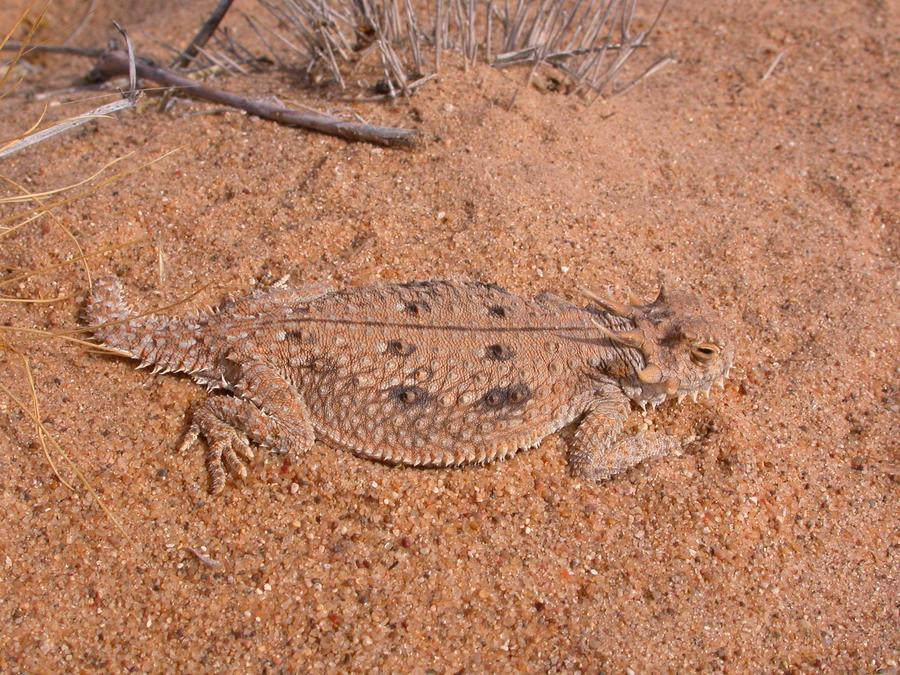
\includegraphics[width=3.6in,height=2.7in]{Ch15-searchencounter/figs/horny_lizard.jpg}
\caption{A flat-tailed horned lizard showing its typical cryptic
  appearance in its native environment.  Detection of flat-tailed
  horned lizards is difficult because they do not run when
  approached. Instead they shuffle under the sand or press down and
  remain motionless as shown in the picture.  The horns are employed
  only as a last resort if the camouflage fails.  {\it Photo credit:
    Kevin and April Young} }
\label{searchencounter.fig.hornylizard}
\end{figure}

It is clear that this uniform search intensity model is a special case
of the more general search encounter model in the sense that the
probability of encounter of an individual is a constant $p_{0}$ {\it
  if} the individual is located in the polygon ${\cal X}$ during
sample occasion $k$, i.e.,
\[
p({\bf u}_{ik}) = p_{0} \mbox{I}({\bf u}_{ik} \in {\cal X})
\]
which resembles Eq. \ref{search-encounter.eq.hardplot} except
replacing the encounter probability function with constant $p_{0}$.


\subsection{Alternative movement models}
\label{searchencounter.sec.movement}

In the analysis of \citet{royle_young:2008}, a simple bivariate
Gaussian movement model was used, in which
\[
 {\bf u}_{ik} | {\bf s}_{i} \sim \mbox{Normal}({\bf s}_{i}, \sigma^{2}{\bf I}),
\]
However, clearly more general versions of the model can be developed.
For example, imagine a situation where the successive urveys of a
bounded sample polygon are relatively close together in time so that
successive locations of individuals are not well-approximated by the
Gaussian movement model, which implies independence of locations. Naturally we might consider using an
auto-regressive or random-walk type of model in which the successive
coordinate locations of individual $i$ behave as follows:
\begin{eqnarray*}
 u_{1}(i,k) | u_{1}(i,k-1) &\sim &  \mbox{Normal}( u_{1}(i,k-1),  \sigma^{2}) \\
 u_{2}(i,k) | u_{2}(i,k-1) &\sim &  \mbox{Normal}( u_{2}(i,k-1),  \sigma^{2}) \\
\end{eqnarray*}
here we use the notation $u_{1}$ and $u_{2}$ for the easting and
northing coordinates, respectively. (to keep from cluttering things up
with too many subscripts we have $i$ and $k$ as parenthetic arguments
here).   In addition, we require that the initial locations have a
distribution and, for that, we might begin with a simple model such as
the uniformity model:
\[
 {\bf u}(i,1) \sim \mbox{Uniform}({\cal S})
\]
which effectively takes the place of the model for ${\bf s}_{i}$ that
we typically use. Under this model, individuals don't have an activity
center but, rather, they drift through space more-or-less randomly
based just on their previous location. See \citet{ovaskainen:2004,
  ovaskainen:2008} for development and applications of similar
movement models in the context of capture-recapture data,
% XX RS: For what exactly? More details on that kind of movement model?
% andy sez: I added a phrase to clarify
and also our discussion of a similar model that
might arise in acoustic surveys (Sec. \ref{poisson-mn.sec.acoustic}).
We could allow for dependent movements about a central location ${\bf
  s}_{i}$ using a bivariate auto-regression 
or similar type of
model with parameter $\rho$, e.g.,
\[
 {\bf u}(i,k) | {\bf s}_{i} \sim   \mbox{BVN}( \rho*( {\bf u}(i,k-1) - {\bf s}_{i} ),  \sigma^{2} {\bf I}).
\]


\subsection{Simulating and fitting uniform search intensity models}

In the \mbox{\tt scrbook} package, we provide a script for simulating
and fitting search-encounter data using the iid Gaussian model and
also the random walk model. We encourage you to adapt these to fit the
AR(1) movement model.  The {\bf BUGS} model specification is shown in
Panel \ref{search-encounter.panel.uniform} for the random walk
situation. In this case
we set
up the run with {\bf JAGS}using the standard commands. We did not specify
starting valules for the missing coordinate locations although we
imagine that JAGS should perform better if we provide decent starting
values, e.g., the last observed location or some other reasonable location.
 We imagine that resource selection  could
be parameterized in this movement model as well, perhaps
using similar ideas to those dexcribed in Chapt. \ref{chapt.rsf}. 

\begin{verbatim}
R CODE FOR SIMULATING THIS SITUATION.....................?

To be inserted
\end{verbatim}


\begin{panel}[htp]
\centering
\rule[0.15in]{\textwidth}{.03in}
{\small
\begin{verbatim}
model{
psi ~ dunif(0,1)
tau ~ dgamma(.1,.1)
p0 ~ dunif(0,1)
sigma.move <- sqrt(1/tau)

# Likelihood
for (i in 1:M){
  z[i] ~ dbern(psi)
  G[i,1,1] ~ dunif(0,16)
  G[i,1,2] ~ dunif(0,16)

   for (t in 2:n.occasions){
## See here I can only make a model for LOCATION
      G[i,t,1] ~ dnorm(G[i,t-1,1], tau)
      G[i,t,2] ~ dnorm(G[i,t-1,2], tau)
# Test whether the actual location is in- or outside the study area. Needs to be done for each grid cell
    }
   for(t in 1:n.occasions){
      inside[i,t] <- step(G[i,t,1]-3) * step(13-G[i,t,1]) *step(G[i,t,2]-3) * step(13-G[i,t,2])
      Y[i,t] ~ dbern(mu2[i,t])
      mu2[i,t] <- p0 * inside[i,t] * z[i]
      } #t
   } #i
N <- sum(z[])
}
\end{verbatim}
}
\rule[-0.15in]{\textwidth}{.03in}
\caption{
{\bf BUGS} model specification for the search-encounter model similar
to Royle and Young 2008 but with a random walk movement model.
help file \mbox{\tt ?search$\_$encounter} in the {\bf R} package \mbox{\tt scrbook}.
}
\label{search-encounter.panel.uniform}
\end{panel}

\subsection{Movement and Dispersal in Open Populations}

In Chapt. \ref{chapt.open} we discuss many aspects of modeling open
populations, including some aspects of modeling movement and dispersal
and the relevance of SCR models to these problems. However, given the
introduction of the search-encounter model above, this is celarly
relevant to modeling movement and dispersal in open populations.  In
particular, the model described in Panel
\ref{search-encounter.panel.uniform} could easily be adapted to an
open population by conditioning on the first, and introducing a latent
``alive state'' with survival parameter $\phi_{t}$. This would be a
spatial version of the standard Cormack-Jolly-Seber model
(Chapt. \ref{open.sec.cjs})\footnote{Some work related to this is
  currently being carried out by our colleagues Torbjorn Ergon and
  Michael Schaub.}.

\section{Designs 3 and 4: Partial Information}


Design 1 and Design 2 (USI) are ideal in the sense that they product
both precise locations of individuals and also a precise
charachterization of the manner in which individuals are encountered
by sampling space. 

We have seen a number of studies that, in an ideal world, would have
generated data of a ``Design
1'' type but, for some practical reason or other reason, the model described
above cannot be used.
 We discuss some of these problems here, which all seem to involve a
 design type 1 but with partial information. We imagine there could be
 3 distinct situations
\begin{itemize}
\item[(a)] search path not recorded, locations recorded
\item[(b)] search path recorded, locations not recorded
\item[(c)] search path not recorded, locations not recorded [but plot of
detection is known]  {\bf Capercaillie}
\end{itemize}

For analysis of these search-encounter designs with partial information,
we think there are a number of options depending on the situation:
For (a) you could always assume uniform search intensity ,
which is probably ok if plots were randomly searched.
It would be useful to do a simulation study to look at how bad that
model is if plots were systematically or randomly searched, and with
heterogeneity in search intensity.
For (b), maybe you could map the locations to the center of each plot,
think of the plot as effective traps, and maybe use the search path
length as a covariate, or some measure of coverage of the
plot. Intuitively, this would be a decent solution of the plots are
small relative to typical home range sizes.
For (c) , same thing -- map the locations to the center of the plot,
but now you don't have a covariate of how much effort when into each
plot.


\subsection{Capricaillie status in Switzerland}

Variations on this theme have appeared in a number of papers.  (1)
\citet{mollet_etal:2012}, who obtained a population size estimate of a
large forest grouse species known as the capracaillie ({\it Tetrao
  urogallus}) in Switzerland.  The base SCR model is the Poisson model
(Chapt. \ref{chapt.poisson-mn}). Forest stands were searched by
observers for scat, which was analyzed for DNA identification of
individuals.  A total of 78 spatial units of a few ha each were
searched.  In this example, forest stands were searched but the search
path data was not available, only the unit in which each scat was
found.  It was searched in an expert manner, and it was believed that
a uniform search intensity model could be reasonable.  Importantly,
the sample units are actually large forest patches on the order of
tens of ha each, but variable in size. Data were {\it not} collected
by coordinates of observations but rather just recorded to the
specific patch in which the observation was encountered. To accomodate
this we defined ${\bf s}_{i}$ to be a discrete random variable taking
on values.  Forest patches were searched for scat which was situation
in which discrete patches of habitat are searched using some method
and it might be convenient (or occur inadvertently) to associate
samples to the patch level instead of recording observation
locations. In this case we might use a model $s[i] \sim dcat(probs[])$
where $probs[]$ are the probabilities that an individual inhabits a
particular patch.

\begin{comment}
\begin{figure}
\centering
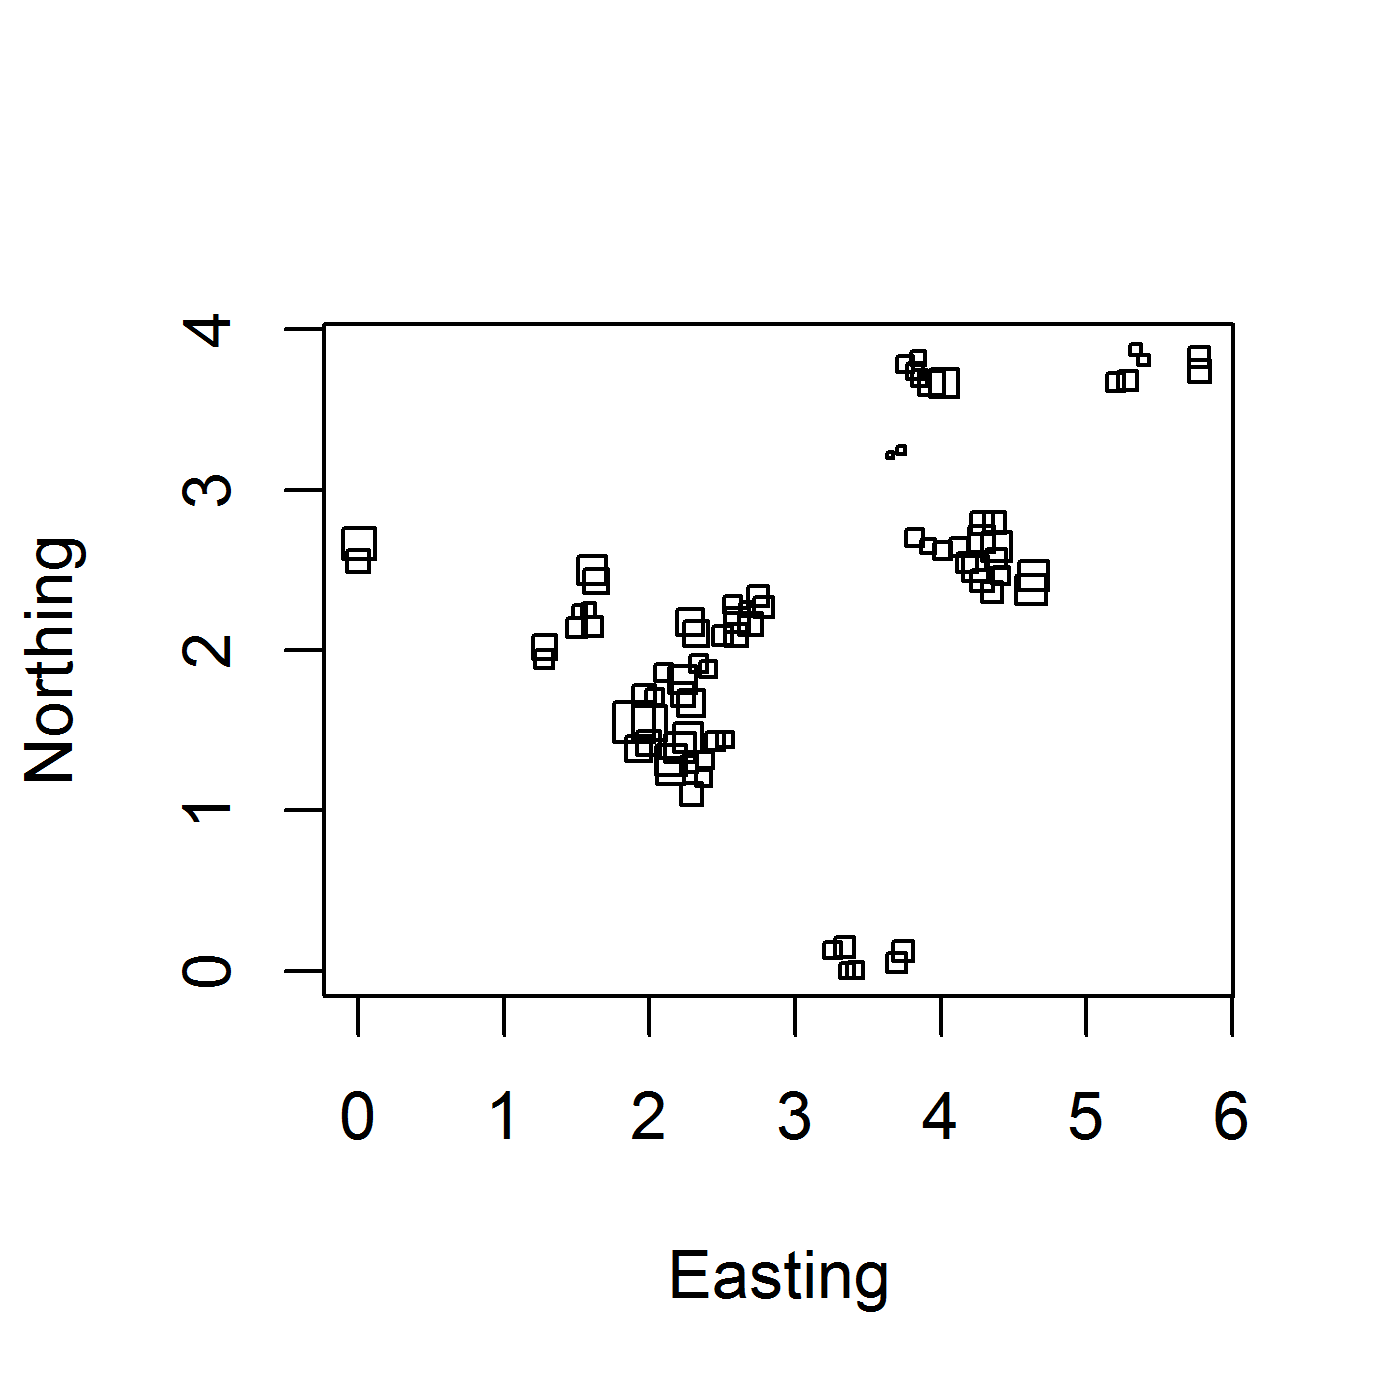
\includegraphics[width=3.5in,height=3.5in]{Ch15-searchencounter/figs/Cap-fragments.png}
\label{poisson-mn.fig.capfrags}
\caption{Relative size and position of 78 forest fragments sampled for
  capricaillie crap.}
\end{figure}
\end{comment}

\begin{figure}
\centering
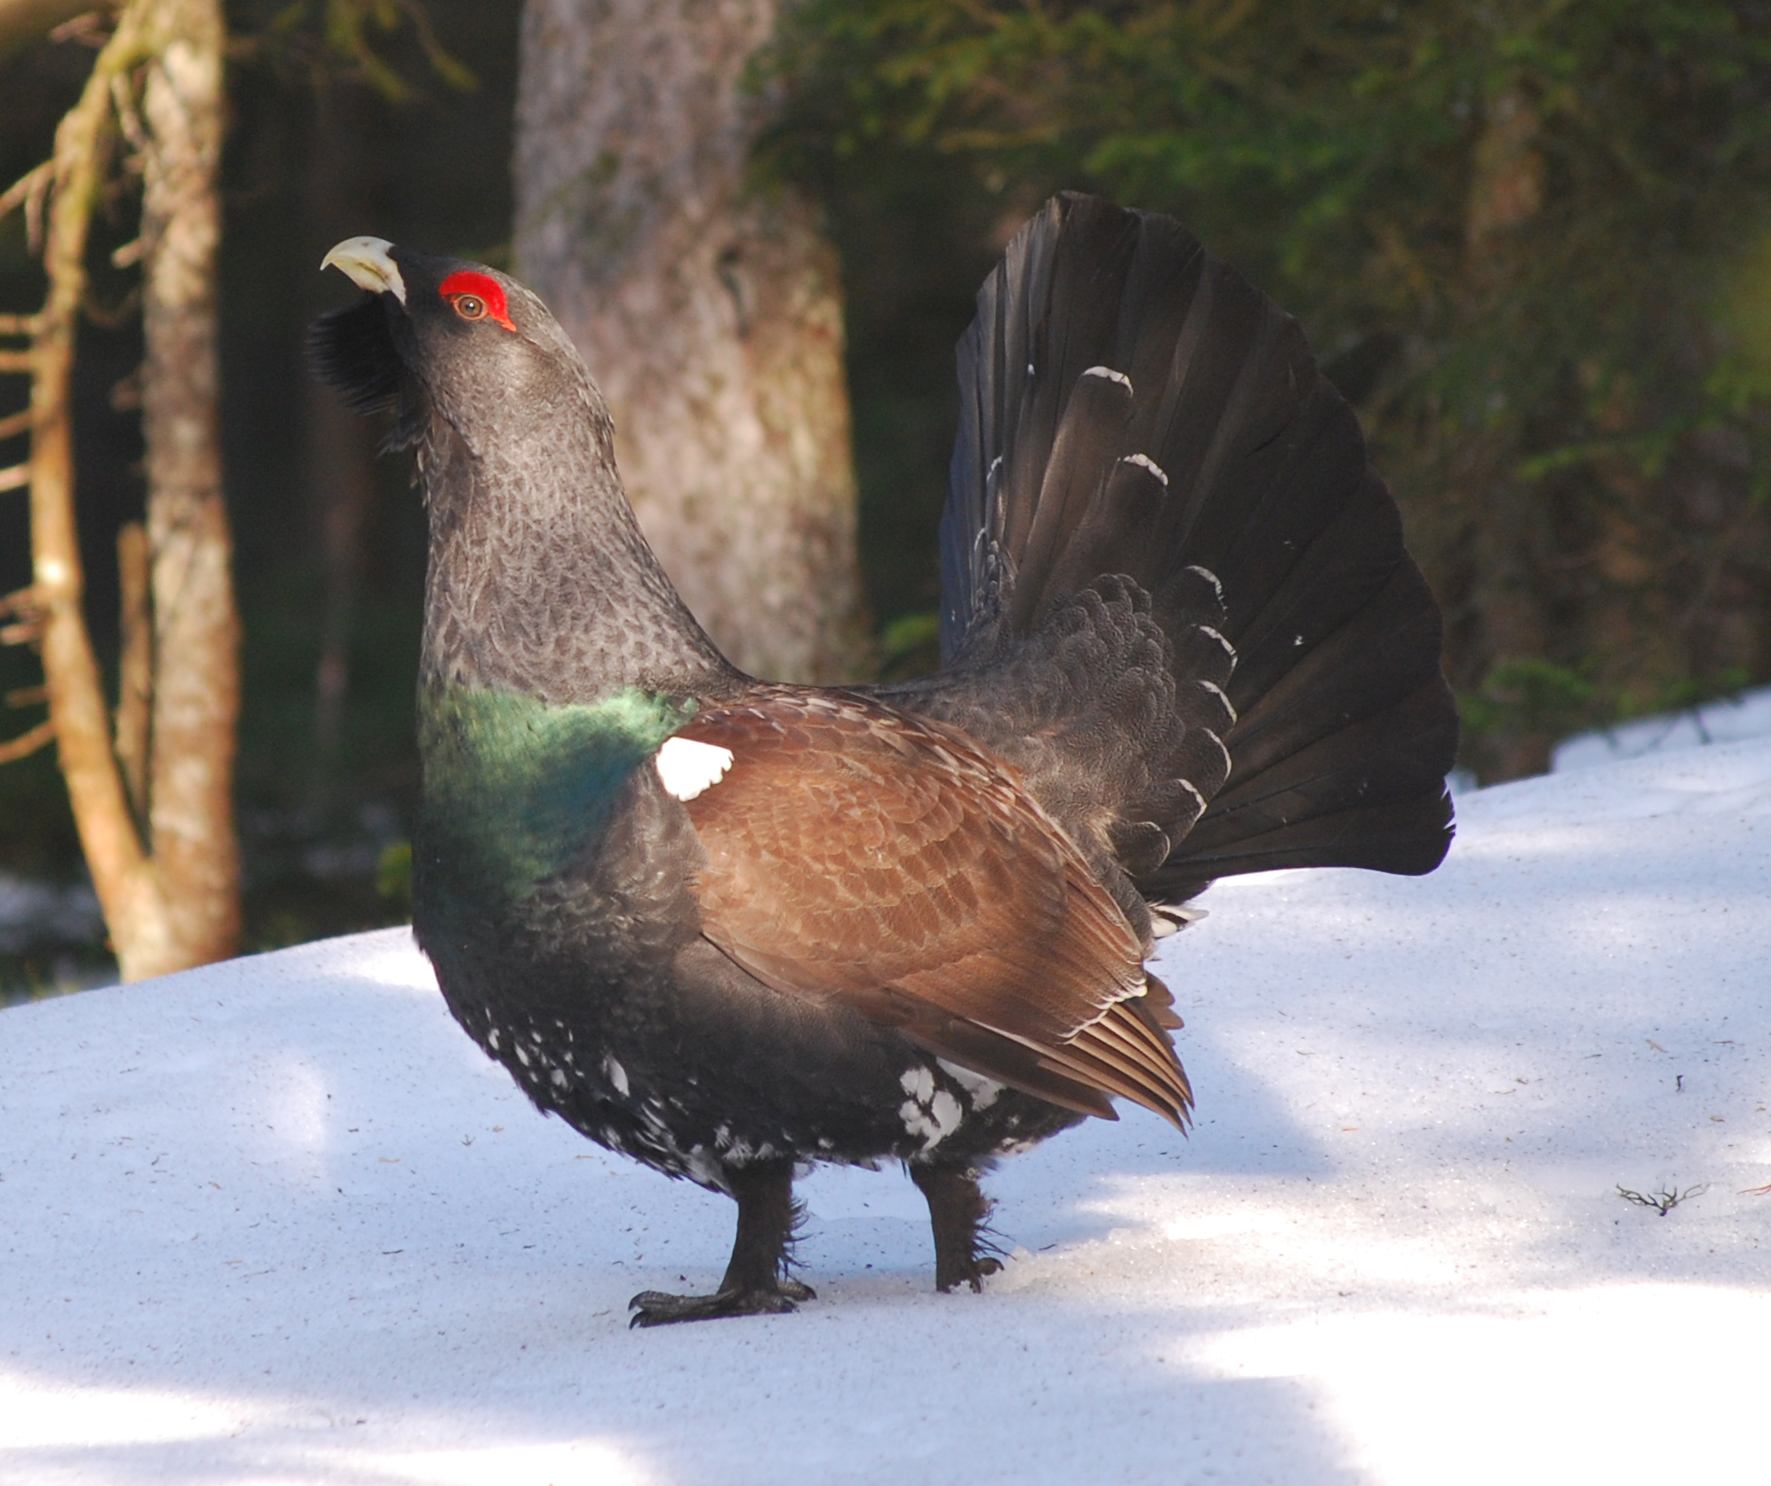
\includegraphics[width=5in,height=4.21in]{Ch15-searchencounter/figs/capercaillie_lanz.jpg}
\label{searchencounter.fig.capercaillie}
\caption{A male caprcaillie in its typical lekking position,
{\it Photo credit: Michael Lanz, Switzerland}.
}
\end{figure}

A key point of the model is that it assumed a discrete model for the
activity centers: activity centers were uniformly distributed to each
of the 78 fragments in proportion to area of the forest patch within
which each fragment was located.  This is similar to the multi-session
formulation of the model where, in this case, the ``sessions'' are
discrete forest fragments but, unlike the multi-session models above,
the encounters of an individual can occur in multiple sessions.  The
authors assumed that
\[
 N_{frag} \sim Poisson( A_{frag} \lambda_{0} )
\]
which implies (see Chapt. \ref{chapt.hscr}):
\[
{\bf s}_{i} \sim  \mbox{Categorical}(  \pi_{frag} )
\]
with
\[
 \pi_{frag} = \frac{ \lambda_{frag} }{\sum_{frag} \lambda_{frag}}
\]
The oservation model: Each of the 78 fragments is its own sample unit which we index to the
center point of the fragment. No finer scale information is made about
the observation locations.
Let $y_{ij}$ be  the number of times individual $i$ encountered in stand $j$.

\subsection{Design 4 -- absence of location information}

We imagine that models can be developed for
situations where we neglect
altogether to record location information within the sample unit.
We see two specific cases here:
Imagine we have a bunch of quadrats or segments that are contiguous or
in close proximity
and we do the surveys like above and record counts PER individual  but
no other sampling information. An example of this is the capericaillie
paper by Mollet et al.....

The other case is that we don't record individual ID at all -- instead
we just have total count frequencies in each plot.
This model is precisely the one considered by
\citep{chandler_royle:2012} and this is the focus of Chapt. \ref{chapt.scr-unmarked}.





\section{Summary and Outlook}

While the use of capture-recapture methods
is commonplace in studies of animal
populations, this includes the classical notion of capture-recapture
based on organized arrays of traps but also a large swath of
``designs'' which are based on organized or haphazard
searches of areas, well-defined or not. For these situations.
Spatial sampling in these ``search-encounter'' situations is distinct
from the classical capture-reapture methods
(e.g., camera trapping) that are based on fixed trap locations.

 In this chapter we showed that SCR models are
relevant to these ``unstructured'' sampling problems in the same way
as ordinary SCR data from trap arrays. One of the key conceptual
points is that, with these search-encounter types of designs, the
locations of observations are {\it not} biased by the locations of
traps but, rather, locations of individuals can occur anywhere within
search plots or quadrats, or in the vicinity of a transect or search
path.  Because we can obtain direct observations of location --
outcomes of movement -- for individuals, it is possible to resolve
explicit models of movement from search-encounter data.  

Key features of what we refer to as ``search-encounter models'' are: 
(1) They contain a model for how space is
sampled, conditional on locations of individuals; and (2) they contain 
a model that
describes how observable animal locations are distributed in space.
We interpret the observable locations as outcomes from a movement
model.  
The models
are somewhat more general than the standard SCR models where
observations are restricted to a priori fixed locations. 

We 
considered the simple case of the independent bivariate normal
movement model, and also a random walk type model, which can easily be
fitted in the {\bf BUGS} engines.  We imagine much more general
movement models can be fitted, although we have had limited
opportunities to pursue this and in most practical capture-recapture
studies, we will probably be limited by sparse data in the complexity
of the movement models that could be consideered. 

We think the search-encounter models will prove to be enormously
useful in future studies of animal populations because so many new
methods of obtaining encounter history data can be be based on DNA
extracted from animal tissue or scat, which is easy to obtain by
searching space and collecting it opportunistically. 


SCR/DS?